\documentclass[12pt,a4paper]{report}
\oddsidemargin=-5.00mm
\textwidth=170.00mm
\topmargin=-10.00mm
\textheight=240.00mm

\usepackage[pdftex]{graphicx}
%\usepackage{refcheck}
\usepackage{natbib}%\usepackage{harvard}
\usepackage{amsmath,amssymb}
\usepackage[blocks]{authblk}
\usepackage{indentfirst}
\usepackage{float}
\usepackage[linktoc=all]{hyperref}
\usepackage{color}
\usepackage{titlesec}
\usepackage{listings}
\lstset{frame=lrbt,xleftmargin=\fboxsep,xrightmargin=-\fboxsep}


%\input{../../../Notes/Preamble.tex}
%\input{latex_path/preamble.tex}
%\input{preamble.tex}

% - particular to this problem (vary easily)

\begin{document}
\title{WIM Description.}

%\author{L.G.~Bennetts\authorcr
%luke.bennetts@adelaide.edu.au}
%\affil{School of Mathematical Sciences\authorcr
%University of Adelaide\authorcr
%Adelaide 5005\authorcr
%Australia
%}

\author{T.D.~Williams\authorcr
timothy.williams@nersc.no}
\affil{Nansen Environmental and Remote Sensing Center\authorcr
Thorm{\o}hlensgate 47\authorcr
5006 Bergen\authorcr
Norway
}

\date{\today}
\maketitle

\tableofcontents
%\section{Introduction}
\chapter{Introduction}

%$\quad$\,\,\,\,
Text.

\chapter{Mathematical and physical background}

Text.


\section{Scattering model}
Text.

\subsection{Two-dimensional model: a single floe}

Text.
\cite{williams-etal2013-break2}
%%%%%%%%%%%%%%%%%%%%%%%%

%\begin{figure}[H]
%\begin{tabular}{cc}
%\includegraphics[scale=0.27]{xtra_figs/foto-conc79-setup.pdf}
%&
%\includegraphics[scale=0.27]{xtra_figs/foto-conc39-setup.pdf}
%\end{tabular}
%\caption{Set-up of the multiple floe experiments, with two different concentrations:  one at a higher concentration, about 79\% (left), and another at a lower concentration about 39\% (right).}
%\label{pic-mult-setup}
%\end{figure}

\chapter{Cron and Crontab} \label{cron}
%\input{CRON.tex}
In this chapter, after a brief introduction on \textit{Cron}, the user will learn how to check and modify a \textit{Crontab} file.
\section{Introduction}
\textit{Cron} is a software utility time-based for \textbf{Unix-like} operating systems. \textit{Crontab} is a text file that guides \textit{Cron} providing the time and nature of its operations; it is possible for every user to have a personal \textit{Crontab}. Every \textbf{minute} \textit{Cron} checks the uploaded \textit{Cronfile} comparing it to the \textbf{system} time. These tasks will run regardless of whether the user is actually logged into the system.
\section{Crontab editing}
The layout of the \textit{Crontab} file (fig. \ref{crnlay}) provides 5 inputs for time and 1 for the command:
\begin{figure}[h!]
\centering
\fbox{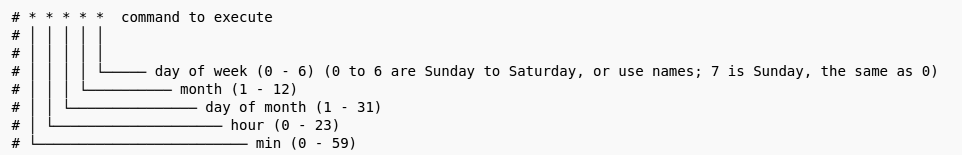
\includegraphics[width=1\textwidth]{crontablayout}}
\caption{\textit{Crontab} file's layout with explanation}
\label{crnlay}
\end{figure}
\begin{lstlisting}[language=bash]
# This is an example of a Crontab file
* * * * * /home/user/prog1.sh	# Every minute
15 * * * * /home/user/prog2.sh	# Every hour at min 15
# Comments don't interfere with Cron
12 18 * * * /home/user/prog3.sh	# Every day at 18:12
*/5 * * 1 * /home/user/prog4.sh	# Every 5 minutes of January
\end{lstlisting} 
\textbf{NOTE} - *\textbackslash \ will reiterate that command \\ \\
To modify the \textit{Crontab} a previously written file can be uploaded (\textit{i.e. mycrontab}) or it can be manually modified (this will change the current user's). \\
\begin{lstlisting}[language=bash]
$ crontab mycrontab 	# Uploading a personal Crontab
$ crontab -e	 	# Manually modifying the Crontab
\end{lstlisting}
\section{Crontab on Hexagon}
\textit{Cron} is working on \textbf{Hexagon} as well but since is a very busy and heavily stressed system there are a few precautions that should be remembered before setting up a \textit{Cron} job. \\ \\
First of all you should choose a \textit{node} in which set up your \textit{Crontab}. A \textit{node} is a connection, redistribution or communication point for a network. For more information please visit (\url{http://docs.hpc.uib.no/wiki/Main_Page}). \\
Another precaution is to use unique \textit{Crontab} file's names so that different set-ups will not be uploaded by mistake. \\ \\
Here is shown a complete procedure for a \textit{Crontab} setup in \textbf{Hexagon}: \\
\begin{lstlisting}[language=bash]
$ ssh hexagon		# Personal login on Hexagon

# Now a Cron-job is appended to a unique tab 
$ echo "* * * * * /home/user/prog.sh" >> prog_cron

$ ssh login1		# Login node1 (change number to change node)
$ crontab prog_cron	# Uploading unique Crontab
\end{lstlisting}
Now every minute \textit{Cron} will execute \textit{prog.sh} from \textit{node1}. \\ \\
\textbf{Remember} that the outputs of \textit{Cron} are shown in a virtual display hence are lost if not saved. It is possible to set up an automatic e-mail service that will save and send to a specified address the outputs by adding the following line in the \textit{Crontab} file:
\begin{lstlisting}[language=bash]
$ MAILTO=user@domain.org
\end{lstlisting}


\chapter{Model's Inputs Updating Procedure}

%%Model's Inputs Updating Procedure

In this chapter the user will be instructed on how to control the scripts used to download and storage the input files that will be used as initial conditions for the WIM model.\\
There are four products that are updated and/or stored daily:
\begin{itemize}
\item TOPAZ - Weekly Restart Files
\item WAMNSEA - Daily Waves 
\item ECMWFR - Daily Weather
\end{itemize}

\section{TOPAZ}
\subsection{Introduction}
\textbf{T}owards an \textbf{O}perational \textbf{P}rediction system for the North \textbf{A}tlantic European coastal \textbf{Z}ones, simply known as TOPAZ is a coupled ocean-sea ice data assimilation system for the North Atlantic Ocean and Arctic. It is the only operational, large-scale ocean data assimilation system that uses the ensemble Kalman filter. This means that TOPAZ features a time-evolving, state-dependent estimate of the state error covariance. \\ \\
In the regional Barents and Kara Sea forecast system (\textbf{BS1}), the TOPAZ (\textbf{TP4}) is used as an outer model in the nested system. Locally the TP4 model runs once a week for an 11 days period, with 9 days forecast, and produce initial and boundary conditions for the regional model BS1.
\subsection{Data Gathering}
The product consist of 3 different files:
\begin{itemize}
\item TP4restart\textit{YYYY\_ddd\_hh}\_mem001.a
\item TP4restart\textit{YYYY\_ddd\_hh}\_mem001.b
\item TP4restart\textit{YYYY\_ddd\_hh}ICE.uf
\end{itemize}
%ADD A BRIEF DESCRIPTION OF WHAT THE FILES ARE
These files are weekly uploaded to the main server of the forecast system, HEXAGON, the supercomputer service at the University of Bergen.
\begin{lstlisting}[language=bash]
$ ssh hexagon
\end{lstlisting}

%Model's Inputs Updating Procedure

In this chapter the user will be instructed on how to control the scripts used to download and storage the input files that will be used as initial conditions for the WIM model.\\
There are four products that are updated and/or stored daily:
\begin{itemize}
\item TOPAZ - Weekly Restart Files
\item WAMNSEA - Daily Waves 
\item ECMWFR - Daily Weather
\end{itemize}

\section{TOPAZ}
\subsection{Introduction}
\textbf{T}owards an \textbf{O}perational \textbf{P}rediction system for the North \textbf{A}tlantic European coastal \textbf{Z}ones, simply known as TOPAZ is a coupled ocean-sea ice data assimilation system for the North Atlantic Ocean and Arctic. It is the only operational, large-scale ocean data assimilation system that uses the ensemble Kalman filter. This means that TOPAZ features a time-evolving, state-dependent estimate of the state error covariance. \\ \\
In the regional Barents and Kara Sea forecast system (\textbf{BS1}), the TOPAZ (\textbf{TP4}) is used as an outer model in the nested system. Locally the TP4 model runs once a week for an 11 days period, with 9 days forecast, and produce initial and boundary conditions for the regional model BS1.
\subsection{Data Gathering - last modification \today}
The initial product consist of 3 different files that will provide initial conditions:
\begin{itemize}
\item \textbf{TP4restart\textit{YYYY\_ddd\_hh}\_mem001.a} - [\textbf{binary data}] initial conditions of the system.
\item \textbf{TP4restart\textit{YYYY\_ddd\_hh}\_mem001.b} - [\textbf{text}] information and instructions for the first file.
\item \textbf{TP4restart\textit{YYYY\_ddd\_hh}ICE.uf} - [\textbf{data}] informations about sea ice (localization, height, etc..).
\end{itemize}
\textbf{NOTE} - file names could change depending on the service \\ \\
%ADD A BRIEF DESCRIPTION OF WHAT THE FILES ARE
These files are weekly uploaded to the main server of the forecast system, HEXAGON, the supercomputer service at the University of Bergen. Are then temporary stored in a working directory that will be cleared every two weeks hence the need of a script that will daily check and if needed archive and transfer the new data. \\
The logic behind the script is to find all the files with \textbf{TP4restart} in their file-name and check their presence in a list of the stored files. If the file is on the list it has already been archived and the script will move on otherwise will automatically add the new files to the list and to the archive (using a \textit{tar} compression protocol). Every operation will write a report on a daily log that will be sent to a selected user (see chapter [\ref{cron}]).
%ADD AN UP TO DATE LIST OF THE SCRIPTS

%\bibliographystyle{plainnum}e
%\bibliographystyle{plainnat}
%\bibliographystyle{klunamed}
%\bibliographystyle{tim}
\bibliography{master}


\end{document}
